\documentclass[final, unknownkeysallowed]{beamer}
\usetheme{RJH}
\usepackage[orientation=portrait,size=a0,scale=1.0,debug]{beamerposter}
\usepackage[absolute,overlay]{textpos}
\usepackage{subcaption}
\setlength{\TPHorizModule}{1cm}
\setlength{\TPVertModule}{1cm}

\title{Deep convolutional networks for protein structure quality assessment}
\author{Georgy Derevyanko, Guillaume Lamoureux}
\institute[CLS]{Department of Chemistry and Biochemistry and Centre for Research in Molecular Modeling (CERMM), Concordia University, Montréal, Canada}
\footer{}
\date{\today}

\begin{document}
\begin{frame}{}

\begin{textblock}{6}(64.5,0.5)

\includegraphics[width=10.0cm]{Logo/ConULogo_K}
\end{textblock}
\begin{textblock}{6}(76.,0.2)

\includegraphics[width=7.0cm]{Logo/CERMM_transparent.png}
\end{textblock}



\begin{textblock}{39.0}(2,6)
\begin{block}{Introduction}
Protein structure prediction remains one of the outstanding challenges in structural biology. 
The progress in this field is assessed during the worldwide competition called CASP \cite{moult2014critical}.
During this biannual event competitors are given the sequences of the proteins whose structures are 
on the verge of being solved using X-Ray crystallography. The goal of contestants is to predict these 
structures.


The key part of all the workflows competing in CASP is the decoy quality assessment.
During this step an algorithm selects the best candidate structure out of the pool of generated candidates (decoys). 
The final success largely depends on the performance during this step.

In this work we propose an algorithm that learns ranking of the protein candidate structures using 
only atomic densities distributions. The key advantages of our algorithm are:
\begin{itemize}
\item It avoids the feature engineering.

other approaches use pre-engineered feature sets. 
Those are fed to a machine learning or optimization algorithm. 
However the process of obtaining the features can be tedious and time consuming. 
Our algorithm predicts the score of a decoy based only on the atomic densities distributions.

\item It can learn from spatial data

electrostatics and solvent are extremely important for protein stability. 
However, this information is not directly accessible to the state-of-art QA methods.
Our approach enables straightforward access to any physical descriptions of a protein structure defined in the 3D space.
\end{itemize}
\end{block}

\begin{block}{Input and model}

The input of the model is a set of atomic densities. 
First we assign atomic types to the heavy atoms of a structure. 
Then we project the density of each atomic type to the corresponding grid. 
The density of each atom is represented as a gaussian. 
The atomic types are inspired by the SYBYL classification.

\begin{figure}[H]
    \centering
    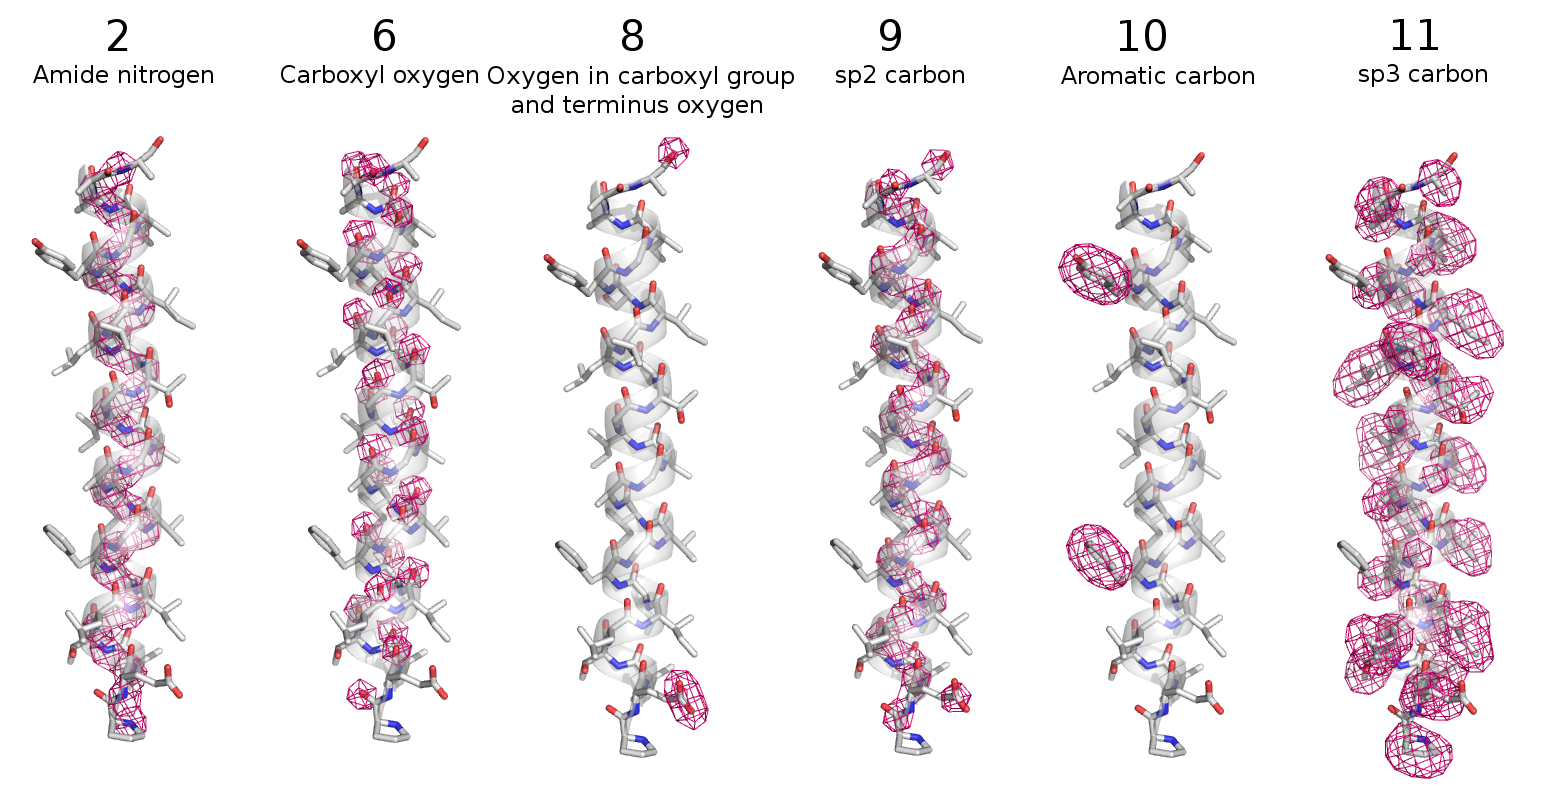
\includegraphics[width=0.7\linewidth]{../draft/Fig/atomic_densities_V3.png}
    \caption{The example of the representation of a protein using atomic densities. The density map is 
    shown using the isosurface at the level $ = 0.5$.}
    \label{Fig:atomic_densities}
\end{figure}

We use convolutional neural network to predict the quality of a candidate protein structure. 
The schematic representation of the model architecture is presented on the figure below.

\begin{figure}[H]
    \centering
    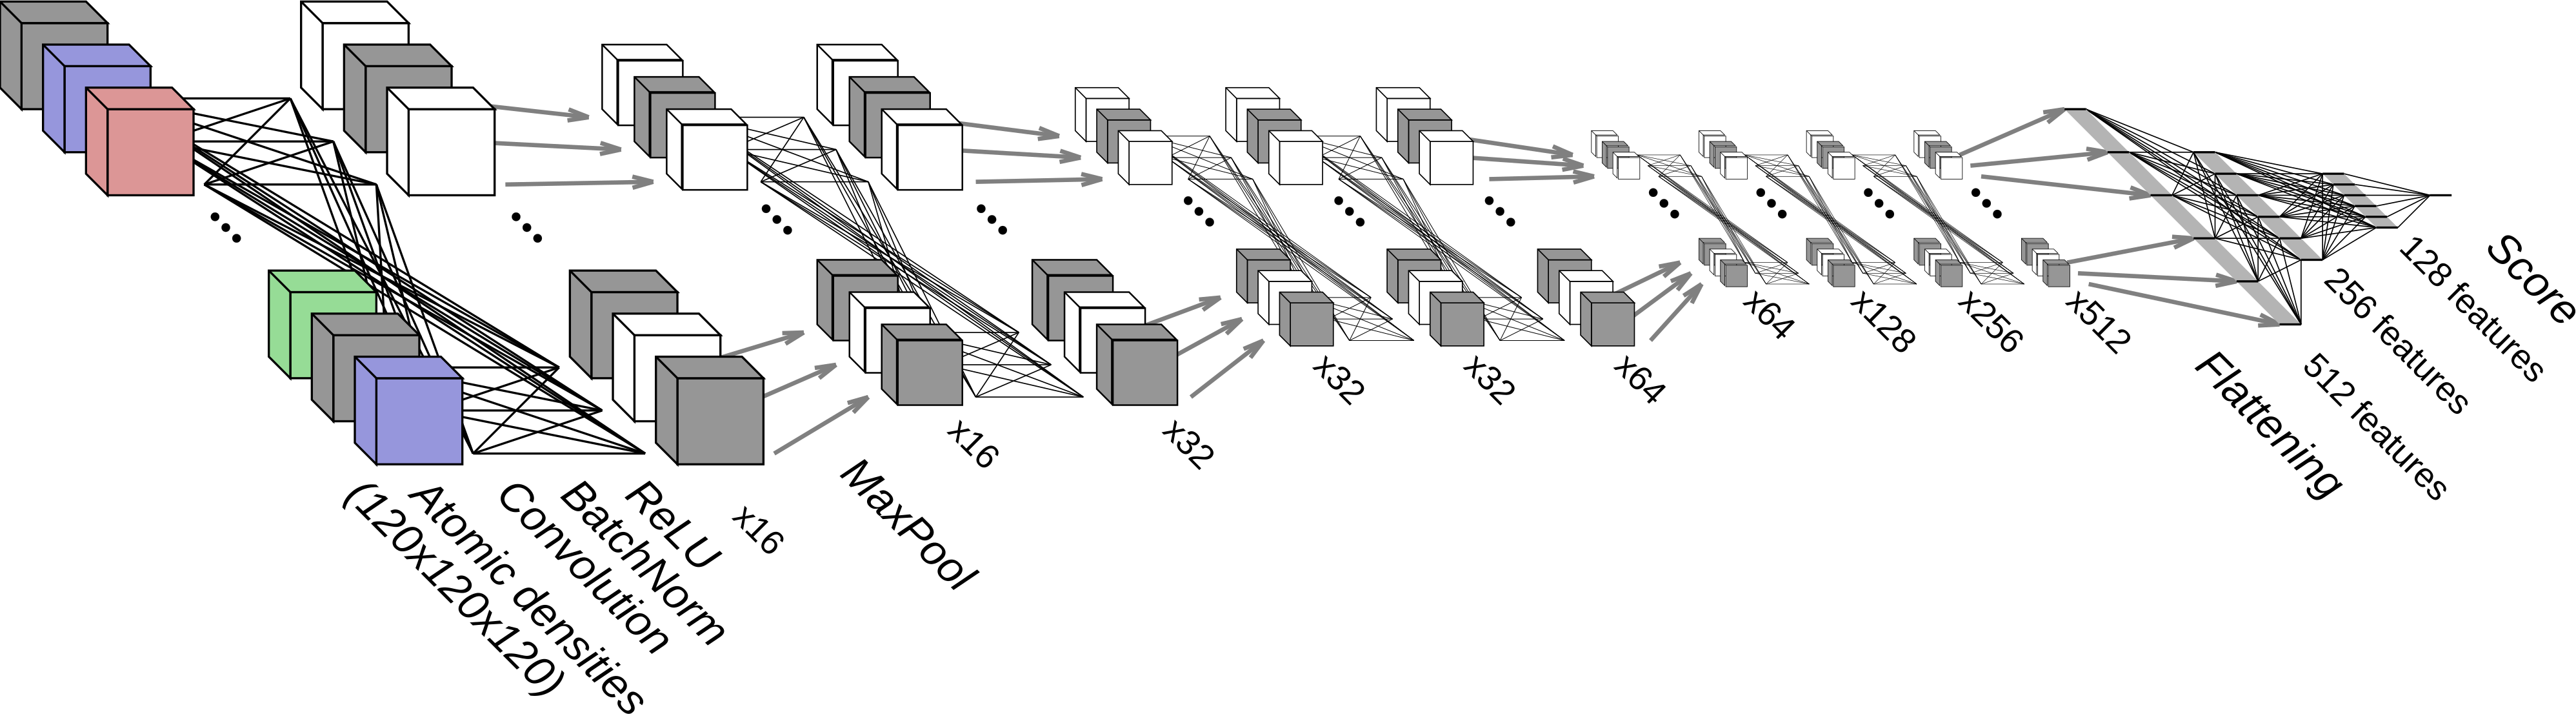
\includegraphics[width=\linewidth]{../draft/Fig/ConvnetDiagramV1.png}
    \caption{The convolutional neural network used in this work. 
    The arrows between the boxes denote maximum pooling layers; the connections denote 
    consequent 3d convolutional, batch normalization and ReLU layers. The $xM$ are the number of filters 
    used in the corresponding 3d convolutional layer.}
    \label{Fig:CNNModel}
\end{figure}

To train the model we use the ranking loss function. 
The ranks for the decoys in the training dataset are defined by the precomputed GDT\_TS scores.
In particular, we use the pairwise ranking loss:
$$ L_{ij} = w_{ij} \cdot \max \left[ 0, 1 - y_{ij} \left( f \left( x_i \right) - f \left( x_j \right) \right) \right] $$
where $w_{ij}$ is zero when the two decoys are too similar and one otherwise. 
The $y_{ij}$ is the coefficient that defines the ordering:
$$
y_{ij} = \begin{cases}
               1& \textrm{GDT\_TS}_i \leq \textrm{GDT\_TS}_j \\
               -1& \textrm{GDT\_TS}_i > \textrm{GDT\_TS}_j \\
            \end{cases}
$$
During the training procedure we optimize the loss function with respect to the parameters of the model.

\end{block}

\begin{block}{Datasets}
   To train and assess our method we used the decoys from previous CASP competitions. 
We took the submissions of contestants during CASP7 - CASP10 as the training set.
The decoys from CASP11 dataset served as the test set.
\begin{itemize}
\item Side chain conformation of the training and test sets were optimized using SCWRL4 program \cite{krivov2009improved}.
\item The training and test sets have 564 and 83 targets correspondingly. Each target in the training dataset has on average 282 decoys.
\item The test dataset is split into two subsets: Stage1 with 20 selected decoys for each target and Stage2 with 150 decoys
for each.
\item The native structures were not included in the datasets nor during the training procedure neither during the testing phase. 
\end{itemize}

Fig. \ref{Fig:foldsGraph} shows the homology between the training and the test sets in terms of 
ECOD structural classification \cite{cheng2014ecod}. 
This information is later used to assess the degree of overfitting of our algorithm.

\begin{figure}[H]
    \centering
    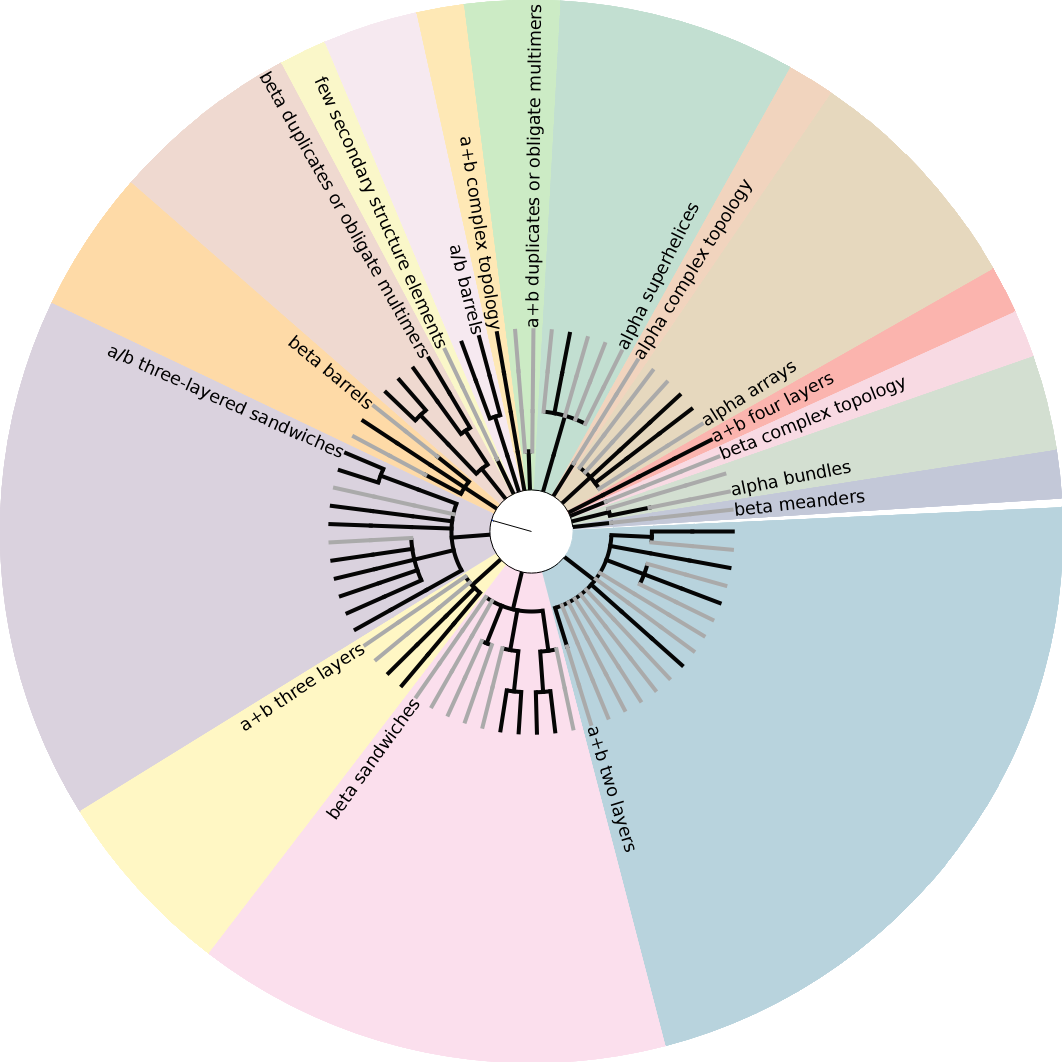
\includegraphics[width=0.50\linewidth]{../draft/Fig/folds_graph.png}
%
    \caption{Classification of the test set structures into the lower
    four ECOD structural levels (from the center out): architecture
    (A), possible homology (X), homology (H), and topology (T). The
    names of the architecture types are shown in the outer circle of
    the diagram.
%%% Why do you have two different architecture names in the same A
%%% group? (brown color: ``alpha complex topology'' and ``alpha
%%% arrays'')
    The grey lines denote test set classes that have no
    respective representative in the training set. The black lines
    show the classes that have representatives in both training and
    test sets. We do not show the F-groups because they have litle
    overlap among the training and test sets.
%%% Why not showing the F-groups?
}
%
    \label{Fig:foldsGraph}
\end{figure}
\end{block}

\end{textblock}


\begin{textblock}{39.0}(43.5,6)

\begin{block}{Results}
To assess the performance of our method (3DCNN) we used different correlation coefficients and the loss criterion.
The former is the deviation of the GDT\_TS of the best decoy from the GDT\_TS of the decoy with the lowest score:
$$ 
Loss = \left| \max_i \left( \textrm{GDT\_TS}(x_i) \right) - \textrm{GDT\_TS} \left[ \textrm{argmin}_i \left( \textrm{3DCNN}(x_i) \right) \right] \right|
$$ 

Table \ref{Tbl:TestResults} shows the comparisson of our algorithm (3DCNN) with the state of art methods: 
ProQ2 \cite{ray2012proq2}, VoroMQA \cite{olechnovivc2017voromqa}, QProb \cite{cao2016protein} and RWPlus \cite{zhang2010novel}.

\begin{table}[H]
\begin{center}
\begin{tabular}{ c | c | c | c | c }
    \multicolumn{5}{ c }{Stage 1} \\ \hline

    QA method & Loss & Pearson & Spearmann & Kendall \\
    \hline
    \textbf{3DCNN}   &0.071 &0.528 &0.414 &0.318 \\
    ProQ2   &0.081 &0.656 &0.534 &0.408 \\
    VoroMQA &0.095 &0.621 &0.504 &0.382 \\
    Qprob   &0.097 &0.631 &0.517 &0.389 \\
    RWplus  &0.128 &0.500 &0.387 &0.291 \\ \hline
    
    \multicolumn{5}{ c }{Stage 2} \\ \hline
    
    ProQ2   &0.058 &0.372 &0.366 &0.256 \\
    \textbf{3DCNN}   &0.067 &0.420 &0.405 &0.285 \\
    Qprob   &0.068 &0.381 &0.387 &0.272 \\
    VoroMQA &0.069 &0.444 &0.437 &0.313 \\ 
    RWplus  &0.095 &0.202 &0.246 &0.175 \\ \hline

\end{tabular}
    
    \caption {Results of our method(3DCNN) and the other state-of-art quality assessment programs on the CASP11 dataset Stage 1 and 2.
            Table shows the absolute, per-target average values of the correlation coefficients and loss.}
    \label{Tbl:TestResults}
\end{center}
\end{table}

\end{block}

\begin{block}{Analysis}
The neural networks are famous for their lack of interpretability. 
Therefore we have to ensure the following:
\begin{itemize}
\item Our model does not overfit 
\item It gives approximatelly the same score for a rotated and translated decoy 
\item It does not rely on some artifacts that can attribute a decoy to a certain contestant, which 
in turn are correlated with the score
\end{itemize}

During the training of the model we augmented the data using random uniform rotations and random translations. 
The Fig. \ref{Fig:DecoysScoreDistribution} shows that the scores under random transformations are distributed approximatelly normally.

To assess the degree of overfitting of our algorithm, we used the classification of targets presented on Fig. \ref{Fig:foldsGraph}
Figure \ref{Fig:LossVsECOD} shows the performance of the algorithms depending on the degree of homology. 
We see, that our algorithm has approximatelly the same performance gains for the homologous proteins as the VoroMQA and ProQ2. 
The algorithm that stands out in this metric is the RWPlus, which seems to be indifferent to the homology. 
However, its performance is also lower than that of the other contenders.

\begin{figure}[H]
    \centering
    \begin{subfigure}{.5\textwidth}
    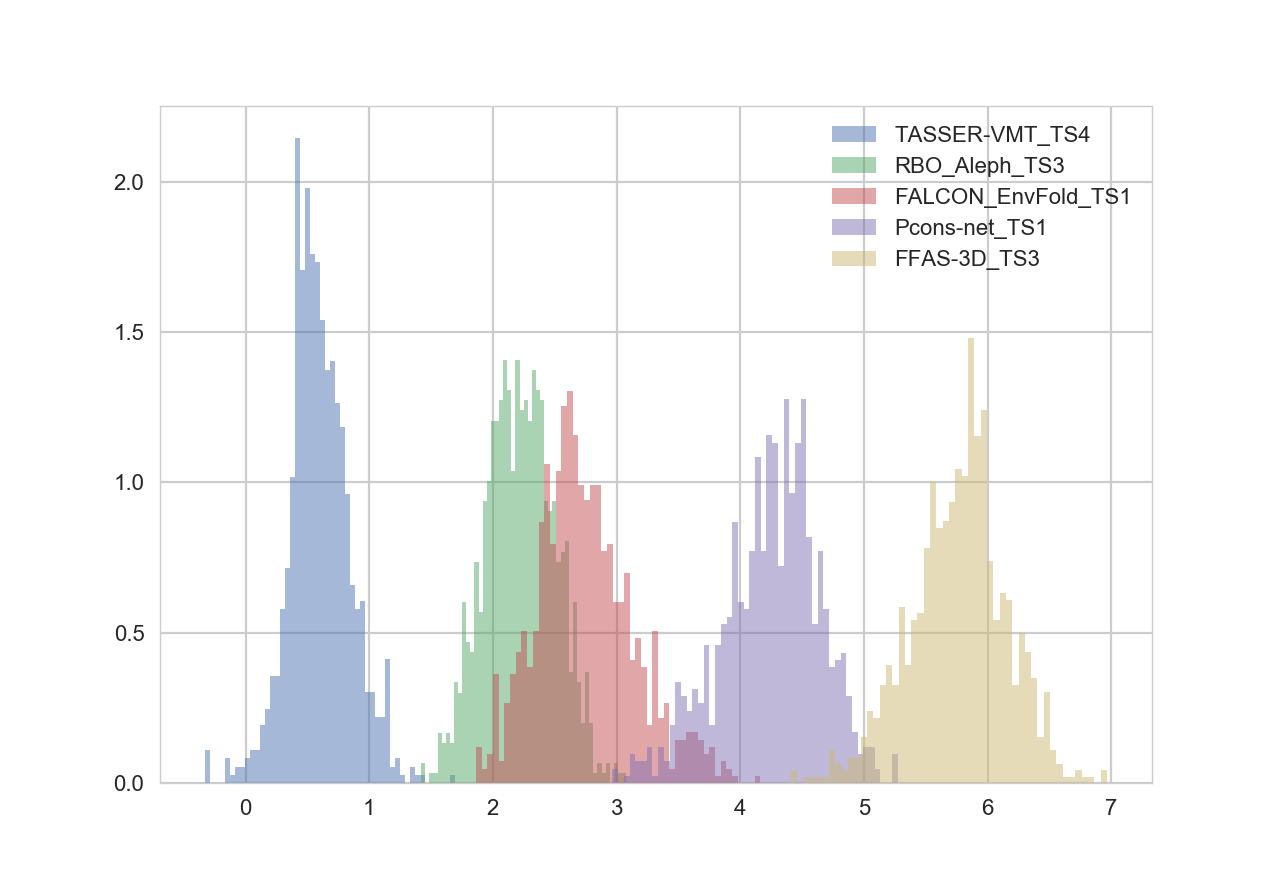
\includegraphics[width=\linewidth]{../draft/Fig/decoys_sampling_dist.png}
    \caption{The distribution of scores under random translations and rotations of several decoys for the target T0832. The 
    names arrangement from top to bottom corresponds to the increase of the score.}
    \label{Fig:DecoysScoreDistribution}
    \end{subfigure}%
    \begin{subfigure}{.5\textwidth}
    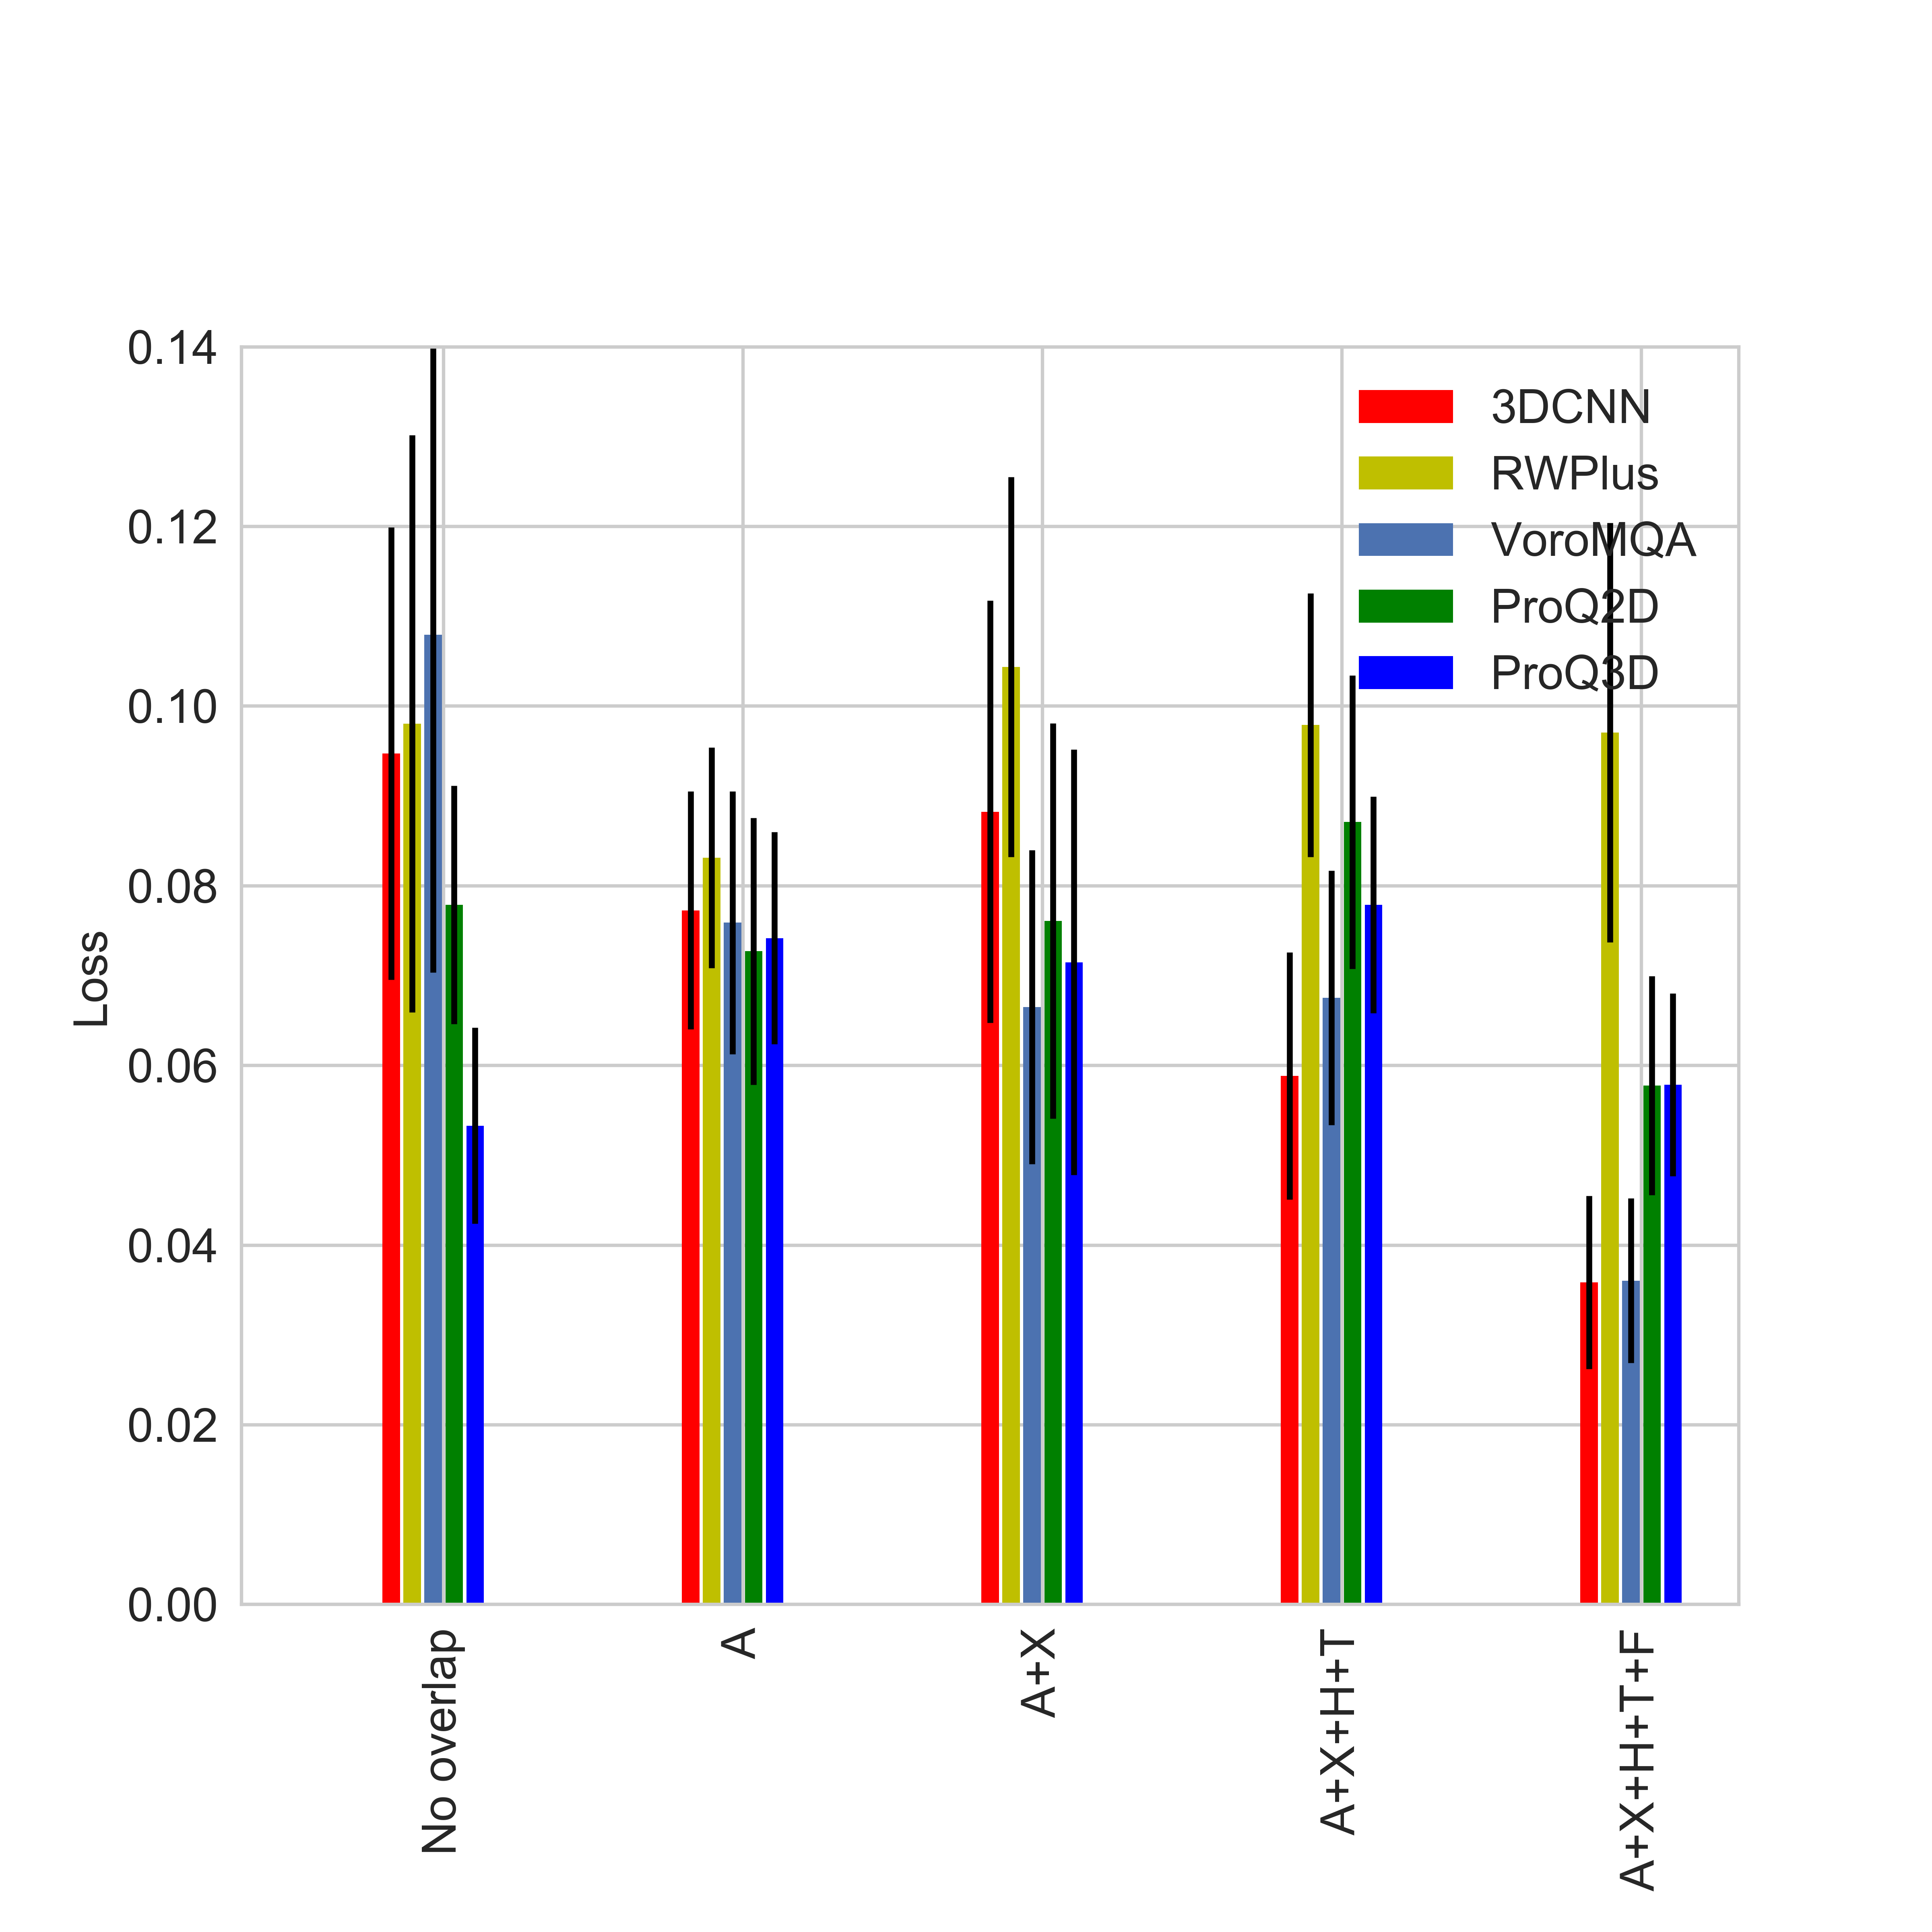
\includegraphics[width=\linewidth]{../draft/Fig/LossVsECOD.png}
    \caption{Loss of different QA-algorithms on the subsets of the CASP11 test set Stage2. The subsets are chosen according to the presense in the
    training set of the structures classified into the same ECOD categories.}
    \label{Fig:LossVsECOD}
    \end{subfigure}
\end{figure}

Finally, to ensure that our algorithm does indeed learn from the structural information and not some artifacts we visualized 
the regions that influense the score the most.
We use the GradCAM method proposed by Selvaraju R. \cite{selvaraju2016grad}. 
It outputs the receptive field, that indicate which parts of the input contributes the most to the positive part of the gradient of the network output.
Fig. \ref{Fig:GradCAMT0776_more} shows the projection of the GradCAM output on the heavy atoms of a protein. 
We see that it highlights the regions at the surface of the protein that are likely misfolded.

\begin{figure}[H]
    \centering
    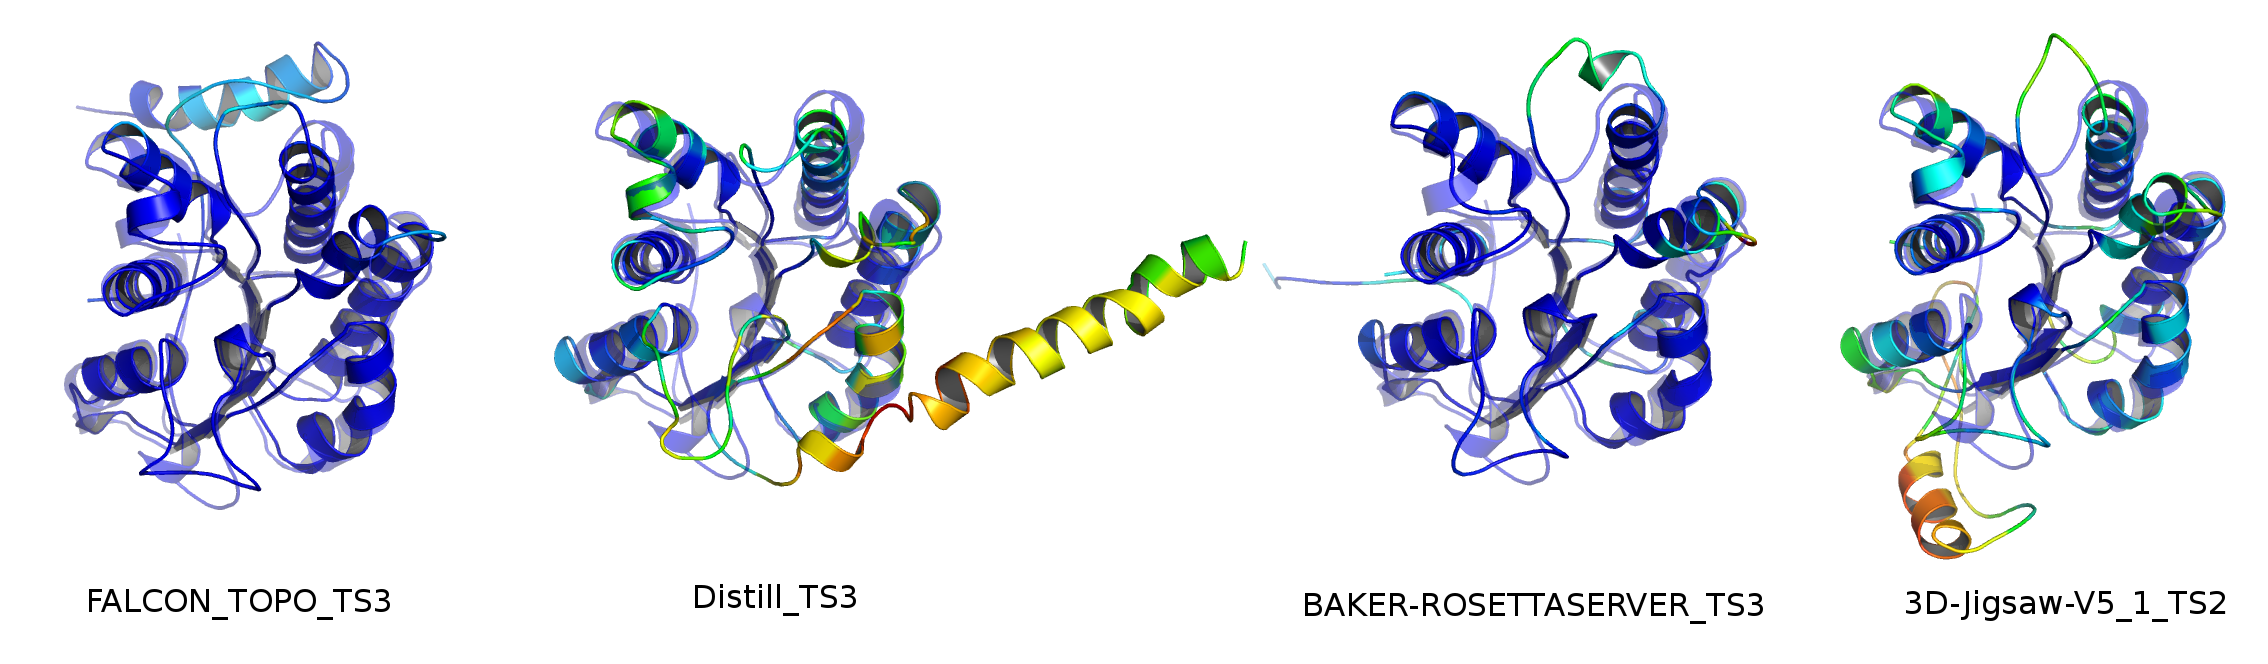
\includegraphics[width=\linewidth]{../draft/Fig/T0776.png}
    \caption{The scaled gradient weighted activation maps of the network projected onto the atoms of the decoys. 
    Each decoy is aligned to the native structure (shown with the transparent cartoon).}
    \label{Fig:GradCAMT0776_more}
\end{figure}

We also verified that the decoys generated by a single algorithm not used in CASP can be successfully ranked by our model.
For this purpose we used 3DRobot dataset \cite{deng20163drobot}. The pearson correlation between the score assigned by 
3DCNN and the GDT\_TS is $0.85$. This indicates, that our algorithm can generalize rather well.

\end{block}




\begin{block}{Acknowledgements}
This research was supported by CERMM grant .
We thank our collaborators from MILA lab for comments and suggestions.
\end{block}

\begin{block}{Citations}
{\small
\bibliography{../draft/citations.bib}{}}
\bibliographystyle{ieeetr}
\end{block}

\end{textblock}

\end{frame}
\end{document}
